%%% template.annotated.tex
%%%
%%% This LaTeX source document can be used as the basis for your technical
%%% paper or abstract. Unlike ``template.tex,'' this version of the source
%%% document contains documentation of each of the commands and definitions
%%% that should be used in the preparation of your formatted document.
%%% 
%%% The parameter given to the ``acmsiggraph'' LaTeX class in the 
%%% ``\documentclass'' command controls several features of the formatted 
%%% output: the presence or absence of hyperlinked icons just prior to the 
%%% first section of the paper, the amount of space left clear for the ACM
%%% copyright notice, the presence or absence of line numbers and submission
%%% ID, and the presence or absence of an appropriate ``preprint'' notice.
%%% 
%%% If you are preparing a paper for presentation in the Technical Papers
%%% program at one of our two annual flagship conferences, held in North 
%%% America (SIGGRAPH) or Asia (SIGGRAPH Asia), you should use ``tog''
%%% as the parameter.
%%%
%%% If you are preparing a paper for presentation at one of our sponsored
%%% events, including SIGGRAPH and SIGGRAPH Asia, but not in those events' 
%%% Technical Papers program, or a one- to four-page abstract, you should 
%%% use ``conference'' as the parameter.
%%% (Technical Briefs and Game Papers presented at our annual flagship 
%%% events fall into this category, as do papers accepted to other SIGGRAPH-
%%% sponsored events, such as I3D or ETRA or VRCAI, as do the one-page 
%%% abstracts which serve as the primary documentation for many of our 
%%% annual conference programs, including Posters, Talks, and Emerging 
%%% Technologies.)
%%%
%%% If you are preparing a version of your content for review, you should
%%% use ``review'' as the parameter. Line numbers will be added to your 
%%% paper, and the submission ID value will be printed across the top of 
%%% each page of your paper. (Use the submission ID as the parameter to the
%%% ``TOGonlineID'' command, below.)
%%%
%%% If you are preparing a preprint of your content, you should use
%%% ``preprint'' as the parameter. This is primarily for annual conference
%%% papers; a header reading ``To appear in ACM TOG X(Y)'' will appear on
%%% each page of the formatted output (where X is the volume and Y is the 
%%% number of the issue in which it will be published).

\documentclass[tog]{acmsiggraph}

%%% Definitions and commands that begin with ``\TOG'' are meant to be used
%%% in the preparation of papers to be presented in the Technical Papers
%%% program at one of our annual flagship events - SIGGRAPH and SIGGRAPH 
%%% Asia. You can safely ignore these definitions and commands if your 
%%% content is to be presented in some other venue.

%%% ``\TOGonlineid'' should be filled with the online ID value you received
%%% when you submitted your technical paper. It will be printed out if you 
%%% prepare a ``review'' version of your paper.

\TOGonlineid{45678}

%%% Should your technical paper be accepted, you will be given three pieces
%%% of information: the volume and number of the issue of the ACM Transactions
%%% on Graphics journal in which your paper will be published, and the 
%%% ``article DOI'' value, which is unique to your paper and provides the 
%%% link to your paper's page in the ACM Digital Library. Fill in the 
%%% ``\TOGvolume,'' ``\TOGnumber,'' and ``\TOGarticleDOI'' definitions with
%%% the three pieces of information you receive.

\TOGvolume{0}
\TOGnumber{0}
\TOGarticleDOI{1111111.2222222}

%%% By default, your technical paper will contain hyperlinked icons which 
%%% point to your paper's article page in the ACM Digital Library, and to 
%%% the paper itself in the ACM Digital Library. You may wish to add one 
%%% or more links to your own resources. If any of the following four 
%%% definitions have URLs in them, an appropriate hyperlinked icon will be
%%% added to the list. 

\TOGprojectURL{}
\TOGvideoURL{}
\TOGdataURL{}
\TOGcodeURL{}

%%% Define the title of your paper here. Use capital letters as appropriate.
%%% Setting the entire title in upper-case letters is not correct, nor is 
%%% capitalizing only the first letter of the title.

\title{The Title of Your Paper Goes Here}

%%% Define the author list in the ``\author'' command. The ``\thanks'' 
%%% field can be used to define an e-mail address for the author.
%%% The ``\pdfauthor'' field should contain a comma-separated list of the
%%% authors of the paper, and is used, along with the title and keyword
%%% data, for PDF metadata. (To see this metadata, open the PDF in Adobe 
%%% Reader and select ``File > Properties > Description.''

\author{Yuhang Li\thanks{e-mail:lyh9001@mail.ustc.edu.cn}\\Xuejin Chen\thanks{e-mail:xjchen99@ustc.edu.cn}}
\pdfauthor{Yuhang Li}

%%% User-defined keywords.

\keywords{geo-localization, point cloud, registration}

%%% End of the document preamble, start of the document.
\usepackage[UTF8]{ctex}%Use Chinese charactors.
\newcommand{\comment}[1]{}
\newcommand{\xj}[1]{\textcolor[rgb]{0.00,0.00,1.00}{(xuejin: #1)} } 
\newcommand{\lyh}[1]{\textcolor[rgb]{1.00,0.00,0.00}{(lyh: #1)} } 
\newcommand{\mdxj}[1]{\textcolor[rgb]{0.50,0.00,0.50}{#1} } 
\newcommand{\lyhpi}[1]{\textcolor[rgb]{0.50,0.50,0.50}{(Paper idea: #1)} } 
\newcommand{\lyhnew}[1]{\textcolor[rgb]{0.30,0.70,0.30}{(New: #1)} } % new content after last review 
\begin{document}

%%% A ``teaser'' image appears below the title and affiliation and above
%%% the two-column body of the paper. This is optional, but if you wish
%%% to include such an image, the commented-out code, below, can be used
%%% as an example. Please note that the inclusion of a ``teaser'' image
%%% may move the copyright space to the bottom of the right-hand column
%%% on the first page of your formatted output. This is acceptable.

%% \teaser{
%%   \includegraphics[height=1.5in]{images/sampleteaser}
%%   \caption{Spring Training 2009, Peoria, AZ.}
%% }

%%% The ``\maketitle'' command uses the author and title information 
%%% defined above, and prepares the formatted title.

\maketitle

%%% The ``abstract'' environment should contain the abstract for your
%%% content -- one to several paragraphs which describe the work.

\begin{abstract}

Duis autem vel eum iriure dolor in hendrerit in vulputate velit esse
molestie consequat, vel illum dolore eu feugiat nulla facilisis at 
vero eros et accumsan et iusto odio dignissim qui blandit praesent
luptatum zzril delenit augue duis dolore te feugait nulla
facilisi. Lorem ipsum dolor sit amet, consectetuer adipiscing elit,
sed diam nonummy nibh euismod tincidunt ut laoreet dolore magna
aliquam erat volutpat.

\end{abstract}

%%% The ``CRCatlist'' environment defines one or more ACM ``Computing Review''
%%% (or ``CR'') categories, used for indexing your work. For more information
%%% on CR categories, please see http://www.acm.org/class/1998.

\begin{CRcatlist}
  \CRcat{I.3.3}{Computer Graphics}{Three-Dimensional Graphics and Realism}{Display Algorithms}
  \CRcat{I.3.7}{Computer Graphics}{Three-Dimensional Graphics and Realism}{Radiosity};
\end{CRcatlist}

%%% The ``\keywordlist'' prints out the user-defined keywords.

\keywordlist

%%% If you are preparing a paper to be presented in the Technical Papers
%%% program at one of our annual flagship events (and, therefore, using 
%%% the ``tog'' parameter to the ``\documentclass'' command), the 
%%% ``\TOGlinkslist'' command prints out the list of hyperlinked icons.
%%% If you are using any other parameter to the ``\documentclass'' command
%%% this command does absolutely nothing.

\TOGlinkslist

%%% The ``\copyrightspace'' command will leave clear an amount of space
%%% at the bottom of the left-hand column on the first page of your paper,
%%% according to the parameter used in the ``\documentclass'' command.

\copyrightspace。


\begin{abstract}
The abstract should summarize the contents of the paper and should
contain at least 70 and at most 150 words. It should be written using the
\emph{abstract} environment.
\keywords{We would like to encourage you to list your keywords within
the abstract section}
\end{abstract}
%
%-------------------------------------------------------
%
\lyhpi{这个问题可以分三个层次(要不要写进论文?或者可以将related work按照这个来写):\\
	1. Alignment:求解overhead image(的edge image)和3D model的竖直投影对齐,假定相机光轴方向与竖直反向对齐。求解只有一个自由度的R,两个自由度的T和一个scale(相当于T的z方向的自由度)。\\
	2. Geo-localization: 找到相机的6DoF pose。3D orientation and 3D location.\\
	3. 2D-3D registration;求解KRT,K的自由度自定,至少包括$f,u_c,v_c$\\
	以上三个层次都可以另外加入一些distortion,如长宽比,剪切比,偏心扭曲等。\\
	}

\lyhpi{目前我们的算法主要解决的是一个geo-localization的问题,求解camera pose(主要)。然后可以用camera pose来求correspondences (未解决),最后用correspondences来做geo-registration问题(非主要)。}
%
%---------------------- Introduction ---------------------------------
%
\section{Introduction}
%
\paragraph{Background/Motivation}
\lyhpi{一开始提data types是为了方便下面existing methods里面按照data type的不同展开。}
Geo-localization has developed rapidly in recent years with the help of powerful sensors which generate a wide variety of types of data, \xj{such as 3D points, dsm??} 
As a key technique to image-based navigation,augmented reality (AR) and 3D reconstruction, geo-localization in urban outdoor environment has drawn massive attentions in the literature.
%
Geo-localization is more challenging than indoor geo-localization because of more complicated environments~\cite{Arth2015a} with more occlusions, more classes of objects and less regular layouts. \xj{explain why outdoor scene is more complicated? occlusions? more classes of objects? no regular shape?}
 %
 \begin{figure*}[!tp]
 	\centering
 	\vspace{2.0cm}
 	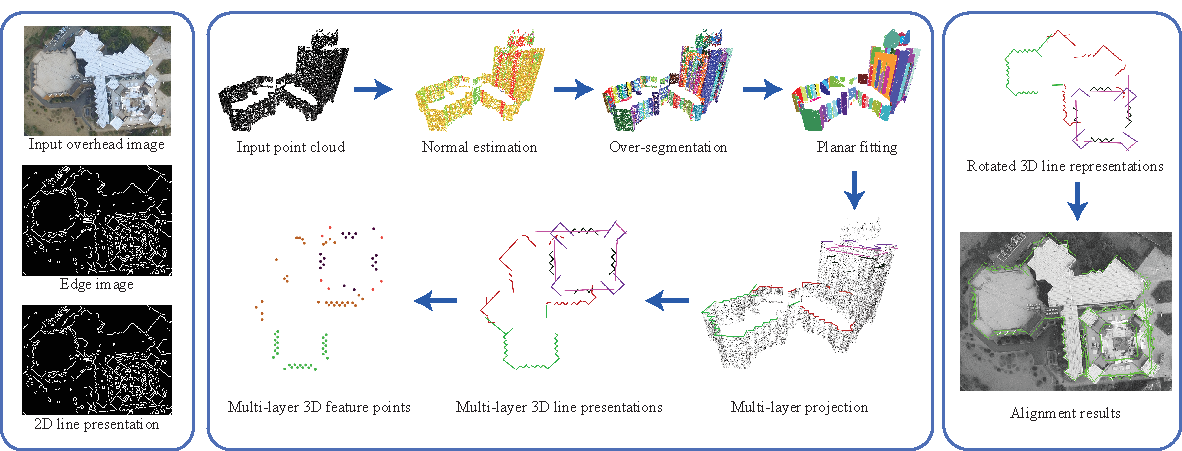
\includegraphics[width=\textwidth]{figures/pipeline_pdf}
 	\caption{Algorithm overview. }
 	\label{fig:overview}
 \end{figure*}
 %
%
\paragraph{Problem statement}
\xj{Do we solve a geo-localization problem?}\lyh{目前paper将问题当做geo-localization问题来解,最后再提及用作初始化解registration问题(这部分没有创新点)}
Outdoor geo-localization aims to compute a large-scale, robust and accurate camera registration in a global coordinate system with metric scale, while it is also different from Simultaneous Localization and Mapping (SLAM) \lyhnew{which does not employ models and therefore presents only relative poses in an arbitrary coordinate system with unknown scale and requires additional motions for initialization \cite{instant}.}
\xj{I don't think this is the key difference. When you say global coordinated system, you just use the 3D model as reference coordinate system. No difference with SLAM. }
\lyh{相比于geo-localzation,SLAM有以下特点:\\
	0. SLAM不需要格外的模型,只要图片/视频,绘制出来的地图是在一个未知的scale下做的。\\
	1. 由于同时做定位和地图绘制,于是定位出来的结果也只是在这个未知scale下的坐标内的位置。\\
	2. 由于是未知坐标,后续为了应用到真实世界,还要在SLAM的基础上加上一个alignment方法才能使用。\\
	3. SLAM要有一个初始化的过程,不然没法自建起一个坐标系统。\\}
\xj{what is the key problem? what is input data and output?}
%
\paragraph{Existing methods and challenges}
When presenting a geo-localization problem, an image or a frame of video is often used as the query data, a 3D model is needed to provide a global coordinate, \lyhnew{a sensor prior is optionally employed, }and the camera pose with respect to the global coordinate system is to be estimated.
\\
\lyhpi{下面这段按照image的不同,简单讨论了现有的方法}\\
%回头确认这几个方法是不是都用了消失点
Some methods capture images or videos by cameras on mobile phones~\cite{Arth2015a, instant, Poglitsch2015, Liu2012} or vehicles~\cite{Taneja2015} on the ground, which are able to take advantages of perspective to compute the camera pose by estimating vanish points. %加一句评价,讲讲消失点很有用
Moreover, some other methods utilize the aerial devices, such as satellites and air plane, to take overhead images at high altitudes, which align the roofs of buildings in images with respect to 3D models (often 3D point clouds), assuming that building roofs in one overhead image captured in high altitude are of a same scale\lyh{有着相同的scale} and therefor projecting 3D models along the vertical vector to generate the global coordinate systems. When it comes to low altitude, perspective effect is more critical, making it a more challenging problem.
\\
\lyhpi{下面这段按照global coordinate system的不同,简单讨论了现有的方法}\\
To obtain the global coordinate system \xj{why to obtain coordinate system?}, some \cite{} maintain databases of pre-registered multiple images. These methods limit themselves while having to collect numerous images covering target areas otherwise only popular spots are available. Another way is employing 3D models, such as digital surface models (DSMs)~\cite{} and 3D point clouds~\cite{}.
\\

\lyhpi{下面提及点云的获得方法和特点来解释为什么要选择用shape matching方法}\\
To acquire 3D point cloud data, a common approach is structure-from-motion (SfM) method\cite{} which is convenient requiring only a series of images to recover a point cloud of a scene. The LiDAR sensor in air plane provides a large-scale but low-quality point cloud\cite{}. 3D models comprising with millions of points can be generated by ground laser scan devices, which provide highly accurate and dense data with metric scaling. However, these laser devices usually fail to capture buildings roof while only vertical facades of buildings are scanned.
\xj{highlight: Missing of roof data makes the registration problem of bird-eye view and 3D models significant challenging.}
\lyh{To be solved}
%
More recently \cite{instant} presents a novel technique that use an untextured 2.5D map (2D map and height) which is \comment{unavailable in some cities and } inaccurate in details.%在很多cities,建筑的2D map都不准确 
\xj{3d models are also unavailable for many cities...}
%
\paragraph{Our key idea and contributions}
\xj{ To solve what problem, we present our method? }
%
In this paper, we present a novel algorithm to \lyhnew{geo-localize the camera of} an overhead image captured by a quadrotor in a low altitude by computing the 6-Dimension-of-Freedom(6DOF) camera pose of the image with respect to the point cloud model coordinate of metric scale. 
%
At first, we treat this problem as a shape matching problem between the edge image of the overhead image and the 2D line presentation of the point cloud \lyhnew{to generate an initial pose for subsequent steps.}
\xj{why use shape matching? what kind of properties will solve the above problem?}
%
We obsolete the high-altitude assumption that building roofs in overhead images are of same scales and propose a novel multi-level strategy to handle low-altitude overhead images where assign different scales to roofs in different heights. 
Moreover, once we achieve the shape matching results we determine the correspondences by matching corners of images with feature points of point clouds. 
At last, we geo-register these two types of data using sparse bundler adjust (SBA) algorithm. 

\lyhnew{\lyhpi{contributions}
To sum up, the contribution of our paper is three-fold. 
At first, we introduce a novel multi-level strategy to handle the low-altitude image. 
Moreover, 
At last,}


%------------------- Related work ------------------------------------
%
\section{Related work}
In this section a brief review of existing approaches on Geo-localization is given...
%
\xj{more references are needed.}
\subsection{Geo-localization with image database}

With a large dataset of pre-registered images, image-based methods compute 6DOF camera pose of a given image. 
\cite{Schindler2007} maintains a dataset of streetside images and uses a vocabulary tree to recognize the location. 
A wide-baseline matching algorithm is presented by \cite{Robertson2004} to identify corresponding building facades generated from a image dataset in two views. It can handle significant changes of viewpont and lighting. \cite{Zamir2014} applies a multiple nearest neighbor feature matching method with a local feature constraint. 
%
\xj{In comparison, we do what?}


\subsection{Geo-localization with models}
\cite{Kaminsky2009} aligns a SfM model of urban environment to a corresponding overhead image by computing an objective function that matches 3D points to image edges under a free space (space without buildings) constraints based on the visibility of points in each camera. 
They use not only the points of SfM model but also the camera poses of images which are both generated from image collection.
\cite{Crews2013} geo-registered 3D point clouds to a scaled map image by defining a normalized Hough similarity function and aligning planes (i.e., walls) in 3D point clouds to lines in 2D maps.
\cite{ECDM} treats the geo-localization as a shape matching problem and aligns 2D the vertical projection of the 3D building roofs and edges of satellite images. An extended Chamfer matching is used to handle noise and occlusions while a global constraint is introduced to optimize the alignment within a large region.
%
In comparison, our method applies a fast version of Chamfer matching algorithm~\cite{FDCM} to \textbf{accelerate} the process where the matching algorithm is based on line segments instead of \mdxj{dense} points used in \cite{ECDM}, and introduces a multi-level strategy to handle low-altitude overhead images where we assign different scales to roofs in different heights. 
%
\subsection{Geo-registration}
...
%
%
%------------------------- Overview ------------------------------
%
\section{Overview}
%<point cloud, line, facades, roofs等等的单复数问题>
%那些数学符号要用黑体、斜体、花体?
%{Assumption: 相机光轴align vertical vector。}
%{其实不是每个点都满足这个投影公式的,只有对应点满足。但是在找到对应点之前的Alignment问题里面也要用到}
%{要不要改成齐次坐标?}
Given a 3D point $(x,y,z,1)$ of the point cloud model, and a 2D point $(u,v,1)$ of the overhead image captured by a quadrotor in a low altitude, our goal is to compute the transform matrix $\mathbf{RT}$ projecting the 3D the point to the 2D point using 
%
\begin{equation} \label{eq:problem}
m\begin{bmatrix}
u\\v\\1
\end{bmatrix}
= \mathbf{K} \mathbf{RT}
\begin{bmatrix}
x\\y\\z\\1
\end{bmatrix},
\end{equation}
%
where $m$ is the normalization term ensuring the third dimension of the 2D point to be one, $\mathbf{K}$ is the pre-calibrated intrinsic matrix of the camera, $\mathbf{R}$ is the rotation matrix and $\mathbf{T}$ is the translation matrix.

\xj{do you calibrate the camera intrinsics? how? }
\xj{three main steps: extraction of feature point correspondences, ..., as Fig~\ref{fig:overview} shows.}
Our algorithm consists of three main steps as Fig~\ref{fig:overview} shows. At first, we treat this problem as a shape matching problem between the edge image of an overhead image and the 2D line presentation of a point cloud where we assume that the optical axis of the camera aligns to the gravity direction and apply a novel multi-level projection strategy to handle the low-altitude problem. Moreover, we determine correspondences by matching corners of images with feature points of point clouds. At last, these two types of data are registered with the correspondences using sparse bundler adjust (SBA) algorithm.


\xj{Explain every variable and every key elements with equations or mathmatical symbols. In order to solve RT, what things should be known?}
%
%------------------------- Shape matching ------------------------------
%
\section{Shape matching}
%
Our building point clouds are obtained by scanning buildings using a ground laser equipment. Only vertical facades of buildings, walls, are captured, and roofs are not able to be scanned by the ground equipment, as Fig~\ref{fig:overview}~(a) shows. 
The overhead images are captured by a quadrotor in a low-altitude. We assume the optical axis of the camera aligns the camera aligns to the gravity direction. This assumption will be discarded in Section~\ref{sct:geo-registration}.
The fact that vertical facades of a point cloud correspond to lines of building roofs in the overhead image \cite{ECDM} inspires us to project the point cloud along the vertical vector and to treat this geo-localization \lyh{ Geo-localization?} problem as a shape matching one in this stage. 
In this kind of problem, one or multiple templates and a target image are needed. 
We generate the 2D templates by projecting the point cloud with a multi-level strategy and apply the edge image of the input overhead image as the target image.

Let a point in a 2D template be $(u_p, v_p, 1)$ and a point in 2D target image be $(u_e, v_e, 1)$. We compute a rotation matrix $\mathbf{R}_{sm}$ with only one dimensional freedom, a scale $s$ and a translation $\mathbf{T}_{sm}$ with two dimensional freedom subjected to
%
\begin{equation}\label{eq:projection_shape_matching}
m\begin{bmatrix}
u_e\\v_e\\1
\end{bmatrix}
=s\mathbf{R}_{sm}\mathbf{T}_{sm}
\begin{bmatrix}
u_p\\v_p\\1
\end{bmatrix},
\end{equation}
%
where 
\begin{equation}\label{eq:rotation_shape_matching}
\mathbf{R}_{sm}= \begin{bmatrix}
\cos\phi_{z} & -\sin\phi_{z} & 0 \cr \sin\phi_{z} & \cos\phi_{z} & 0 \cr 0 & 0 & 1
\end{bmatrix},
\end{equation}
\begin{equation}\label{eq:translation_shape_matching}
\mathbf{T}_{sm}=\begin{bmatrix}
1 & 0 & 0 & t_x \\ 0 & 1 & 0 & t_y \\ 0 & 0 & 1 & 0
\end{bmatrix}.
\end{equation}
%
\cite{ECDM} projects all pre-scaled and pre-rotated points of a building point cloud model along the vertical vector to obtain the template image and extracts the edge image of overhead image as target image. 
%
Considering that parts of building roofs with different heights are of different scales in a low-altitude overhead image, it is unreasonable to keep the assumption in \cite{ECDM} that the projection scales of all parts of building roofs are the same.  \xj{emphasize this in introduction.}
%
To handle the problem without this convenient assumption, we present a novel multi-height strategy, where we match the point cloud projections of different heights with the overhead image separately. 
%
%
\subsection{Point cloud processing}
%{这一节只是说了how, 没有说why}
A building point cloud,$\mathcal{P}=\{\mathbf{p}_i\}$, $i=1,2,\ldots,N_{Points}$, are pre-processed to get height-related templates for shape matching. 
\paragraph{Normal} If needed, we compute a normal $\mathbf{n}_i$ for each point $\mathbf{p}_i$ in the point cloud using Fast and Robust Normal Estimation (FRNE)~\cite{boulch2012fast} which preservers sharp features such as edges and corners.
%
\paragraph{Vertical direction} The vertical direction of building point cloud should correspond to the gravity direction in the realworld. If needed, the vertical direction can be computed using a Principal Component Analysis (PCA) based algorithm~\cite{KarlNiNicholasArmstrong-Crews2013}. And then, we rotate the point cloud to ensure the third dimension of a point, $z$, presents the height of this point in real world.
%
\paragraph{Segmentation} The point cloud is segmented into clusters $\mathcal{C}_j=\{\mathbf{p}^{j}_i\}$, $j=1,2,\ldots,N_{Clusters}$ by iterated region growing from a randomly selected point with points that are within a Euclidean distance of $\rho$ and a normal difference of $\tau$. This process expands to new adding points repeatedly until every point is assigned to clusters.
% planar fitting 好像对算法没有用
\paragraph{Planar fitting} We fit a vertical plane to each cluster. 
More specifically, for each cluster $\mathcal{C}_j$, we use a RANSAC plane fitting algorithm in PCL~\cite{} to fit a finite planar whose normal is constrained to be orthogonal to the vertical vector. The boundary of each planar is the alpha shape of points. 
\paragraph{Selected heights} A histogram is built, whose horizontal axis represents the height in meter from zero to the building height and the vertical axis presents the number of particular points. To be specific, we find the maximum height $h^{max}_j$ of points in a cluster $\mathcal{C}_j$ and assign this cluster to one of bins of the histogram, $B_k$, $k=1,2,\ldots,N_{Bins}$, making sure that this bin contains $h^{max}_j$ in its height range. And then, for each bin, we sum up point numbers of clusters assigned to the bin as its value. Top $n_{s}$ bins with maximum values are selected, indicated as $B^{selected}_l$, $l=1,2,\ldots,n_{s}$, and the weighted average height $h^{selected}_l$ of each $B_l$ is computed by
%
\begin{equation}
h^{selected}_l = \sum_jInd(j,l)w_jh^{max}_j,
\end{equation}
where $Ind(j,l)$ is a indicator which equals to $1$ if $\mathcal{C}_j$ is assigned to $B^{selected}_l$, otherwise equals to $0$, and $w_j$ is the weight which equals to the number of points in $\mathcal{C}_j$.
%
\xj{Show figures about this step. }
\begin{figure}
	\centering
	\vspace{3.0cm}
	\caption{Contour extraction from point clouds. }
\end{figure}
%
\subsection{sensor pose}
...
%
\subsection{Shape matching}
%前面要说清楚把什么当作template 什么当作target 下面的陈述可以带上数学表达
%没有提及sensor pose
At this stage, we treat the registration problem as a shape matching problem. In a shape matching problem two edge images are needed, a template image and a target image, and we should find a rigid transformation to fit the template image with respect to \lyh{ a part of ?} the target image. To find the rigid transformation, we find the scale, the orientation and the translation respectively. 
%
\paragraph{Scale}The scale between the overhead image and the real-world building (also between the overhead image and the metric-scale point cloud) is easy to compute using the intrinsic parameters and altitude parameter from the aircraft sensors, which is accurate enough for later processing. \lyh{Mathematical language?}
%
\paragraph{Orientation}The camera orientation of the overhead image is equal to the alignment rotation between overhead image and point cloud projection image. A Hough transform based algorithm \cite{Censi2005} is utilized, which is designed to compute the alignment rotation between two edge images, here, a template image and a target image. This algorithm is based on the fact that  a rotation with specific angle of an image in space domain result in a translation along the angle axis in Hough transform domain.
%
\paragraph{Translation} 
Chamfer distance matching is a classical shape matching technique, which sweep every possible transformation with brute force to compute costs between the transformed template image and the target image. 
It can handle all respects of transformation including scale, rotation, inspect and translation. However, chamfer distance matching could be extremely complex in computation and time-consuming. 
In fact, the computation complexity is directly proportional to the search space of \lyh{与搜索空间的每一维的量化个数/粒度成正比}. 
Therefor, we only use chamfer distance matching technique to find the translation while fixing the scale and the rotation to the results computed above and the inspect to one. Also we apply to speed up a fast version of chamfer distance matching algorithm, Fast Directional Chamfer Matching (FDCM)\cite{FDCM}. 
FDCM incorporates edge orientation information in the matching algorithm such that the resulting cost function is piecewise smooth and the cost variation is tightly bounded. %这句话好像没什么用 改表达
Moreover, FDCM is proved to be a sublinear time algorithm using techniques from 3D distance transforms and directional integral images.  %改表达
To compute the transformation, FDCM requires as input two sets of line segments, a template set and a target set, from two input edge images respectively. In \cite{FDCM}, line segments of both two sets are estimated from corresponding edge images using a RANSAC line fitting algorithm. However, the proposal method use the line segments generated in point cloud processing as the template sets.
%{为什么要用point cloud里面的lines来代替原方法的lines?}
%{{Why dont we just use FDCM to compute scale and rotation? Computation complexity?}}
%
\section{Feature point matching}
At this point, 
%
\section{Geo-registration} \label{sct:geo-registration}
%
\section{Experiments}
%
The proposed whole system was tested using our building point clouds and corresponding images. The building point clouds are obtained by scanning buildings using a ground laser equipment around our campus. The images are captured using a quadrone
\section{Conclusion}

%
\section*{Acknowledgements}

To Robert, for all the bagels.

%%% Please use the ``acmsiggraph'' BibTeX style to properly format your
%%% bibliography.

\bibliographystyle{acmsiggraph}
\bibliography{Alignment_of_Model}
\end{document}
